\documentclass[12pt,a4paper]{article}
\usepackage[T1]{fontenc}
\usepackage{natbib}
\usepackage{graphicx}
\usepackage{pdflscape}
\usepackage{amsmath}
\usepackage{caption} 
\usepackage{listings}
\usepackage{xcolor}
\definecolor{codegreen}{rgb}{0,0.6,0}
\definecolor{codegray}{rgb}{0.5,0.5,0.5}
\definecolor{codepurple}{rgb}{0.58,0,0.82}
\definecolor{backcolour}{rgb}{0.95,0.95,0.92}
\renewcommand{\figurename}{Şekil}
\renewcommand{\refname}{Kaynakça}
\usepackage{hyperref}
\date{}
\title{TensorFlow ile Patates ve Mısır Yaprağı Hastalık Seti Üzerinde Eğitilmiş Bir Nesne Tanıma Modelinin C++'a Aktarılması ve Tespitin Gerçekleştirilmesi}
\author{Baranalp Öztürk}

\begin{document}
	\begin{figure}
		\centering
		
\includegraphics{ksbu.jpg}
	\end{figure}
	\maketitle
	
	\begin{center}
		\section*{CNN Modelinin Çalışma Mantığı ve Yapısı}      
	\end{center}
	
	\begin{figure}[h]
		\centering
		\begin{minipage}{\textwidth}
			\centering
			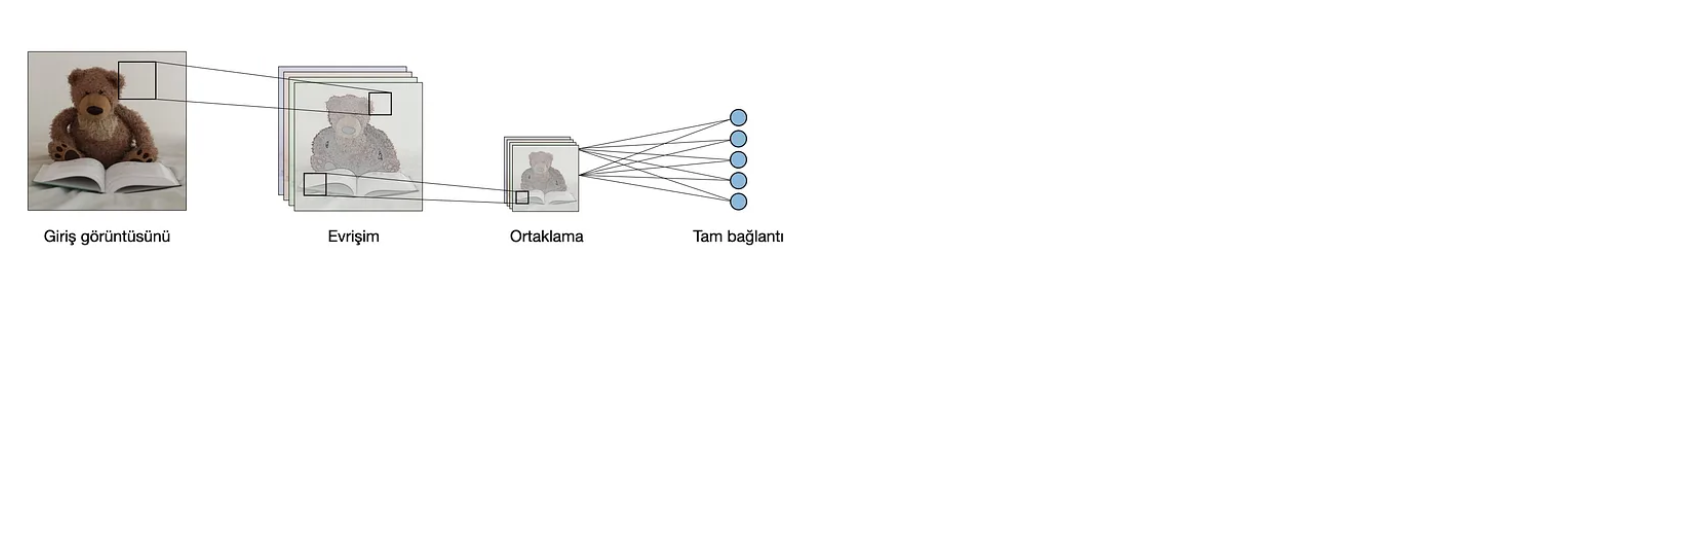
\includegraphics{cnn1.png}
			\vspace{\baselineskip}
			\captionof{figure}{\raggedright En basit şekilde bir CNN modeli görseldeki gibi özetlenebilir. Bir giriş görüntüsü (Input), evrişim katmanı (CONV), ortaklama (pooling) ve tam bağlantı (fully connected — FC) katmanlarından (layers) oluşur.}
			\label{fig:grafik}
		\end{minipage}
	\end{figure}
	
	
	
	
	
	En basit şekilde bir CNN modeli görseldeki gibi özetlenebilir. Bir giriş görüntüsü (Input), evrişim katmanı (CONV), ortaklama (pooling) ve tam bağlantı (fully connected — FC) katmanlarından (layers) oluşur.
	
	\vspace{\baselineskip}
	\pagebreak
	\section*{Katman Tipleri}
	\begin{enumerate}
		\item Evrişim Katmanı (CONV): Bir resme  filtre uygulanarak keskinleştiriliyor ve resmin kenarları daha belirgin hale gelitiliyor.
		İşte bizler CNN’de tamamen rastgele filtreler üretiyoruz, bu rastgele ürettiğimiz filtreleri resmimize uygulayarak resmin belirli bölgelerinden özellik çıkarımı yapmaya çalışıyoruz. Ve yukarıda da fark edebileceğiniz gibi orijinal resmin boyutundan daha küçültmüş yeni bir resimler elde etmiş oluyoruz.
		\begin{center}
			\begin{minipage}{0.65\textwidth}
				\centering
				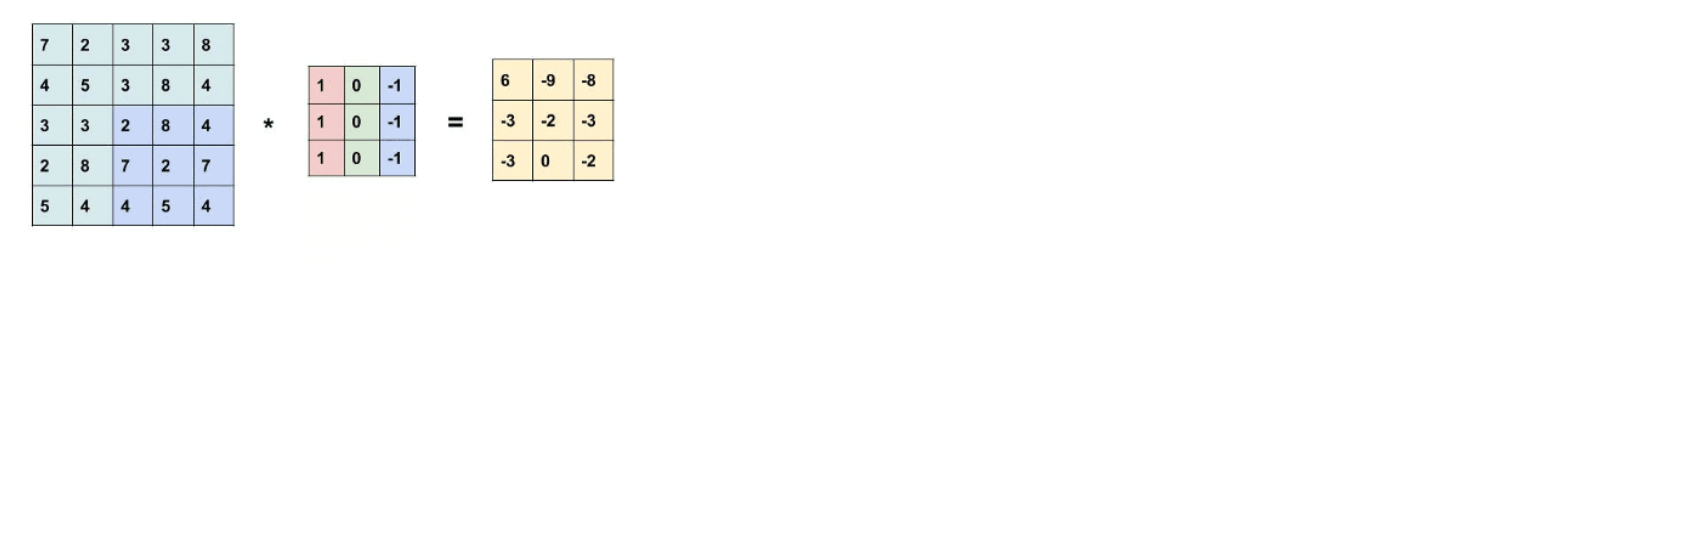
\includegraphics{conver.png}
			\end{minipage}
			\hfill
			\begin{minipage}{0.25\textwidth}
				\centering
				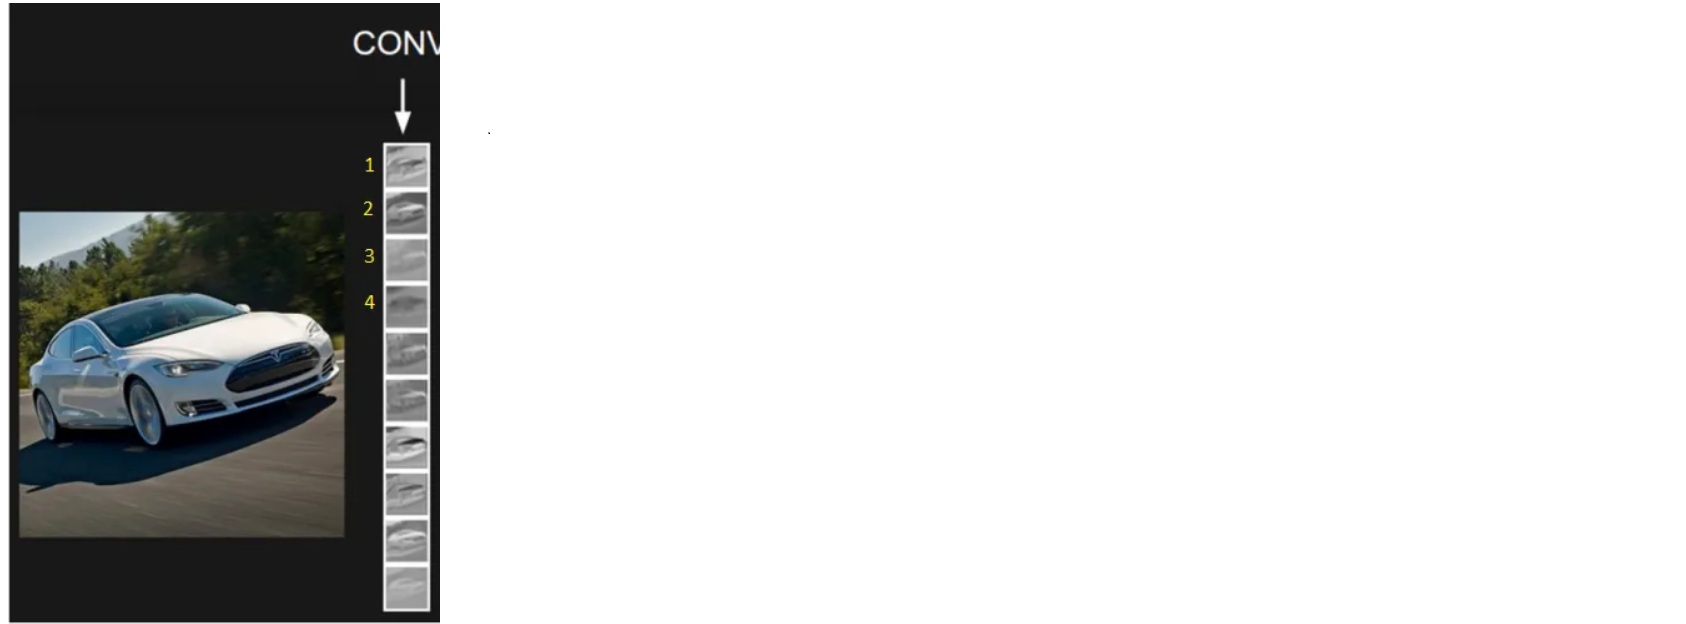
\includegraphics[height=0.5\textheight]{convex.png}
			\end{minipage}
			Orijinal resmimize filtreler uygulayarak elde ettiğimiz 4 tane resim, sarı rakamlar ile ifade edilmiş. Mesela rastgele oluşturulan filtrenin uygulanması ile elde edilen 4. resimde arabanın kaportası daha iyi belli oluyor. 2. resimde ise yol ile arasındaki çizgi daha da ortaya çıkmış.Yani resmin özellikleri ortaya çıkmaya başlamış. Bu resimde biz 3 x 3 ‘lük 10 tane filtre ile çarpım gerçekleştirdik.
			\begin{figure}
				\centering
				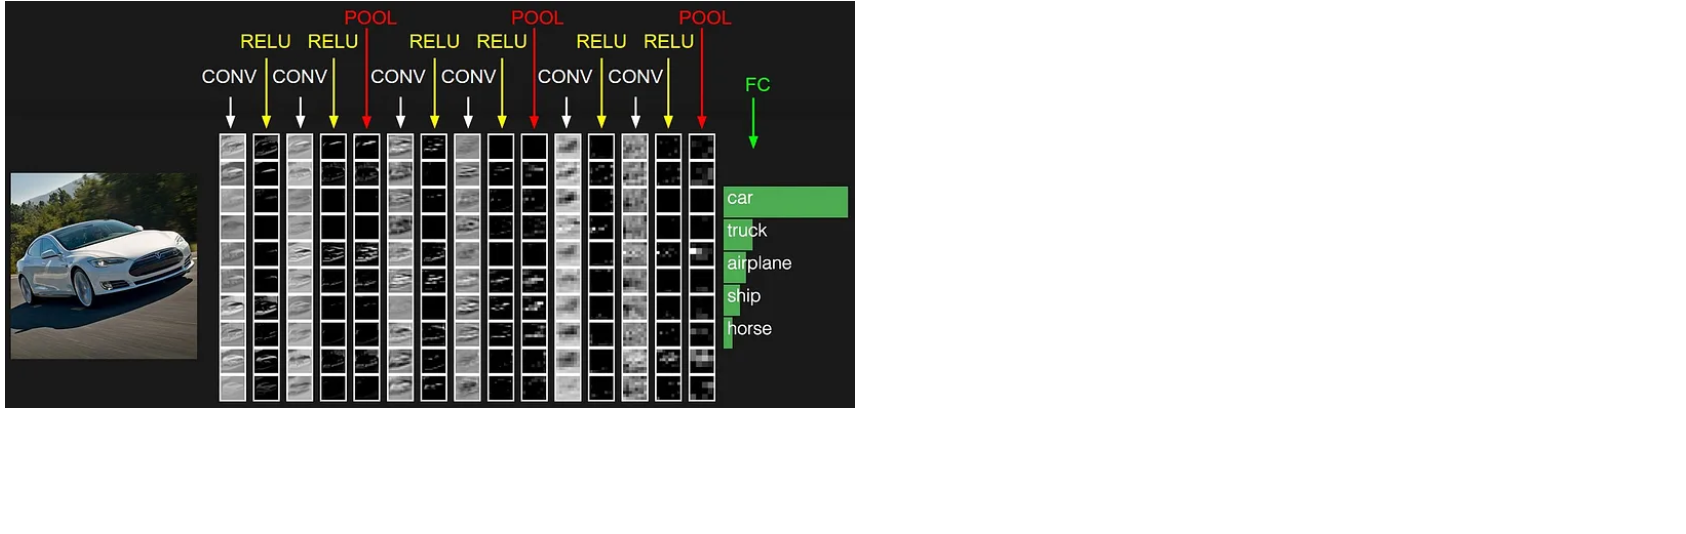
\includegraphics{convex2.png}
			\end{figure}
		\clearpage
		\begin{enumerate}
			\item Pooling: İzmir Saat Kulesi resmi ise 3000 x 2000 piksel. Eğer bu resme 3 x 3'lük bir filtre uygulamaya çalışırsak bizlere büyük sıkıntılar çıkarabilir.
			
			Çünkü bu resme ne kadar evrişim işlemi uygulayabiliriz ki? Günümüz bilgisayarlarının da bir kapasitesi var. Eğer yine de bu resme evrişim işlemlerini uygularsak resmin anlamlandırılması aylar alabilir.
			
			İşte bu sorunu çözmek için Max Pooling işlemi devreye giriyor.
			
			Peki Max Pooling işlemi bizlere neyi sağlıyor?
			
			En temelde resmimizin özelliklerini kaybetmeden boyutunu düşürmemizi sağlıyor.
			
			\begin{figure}
				\centering
				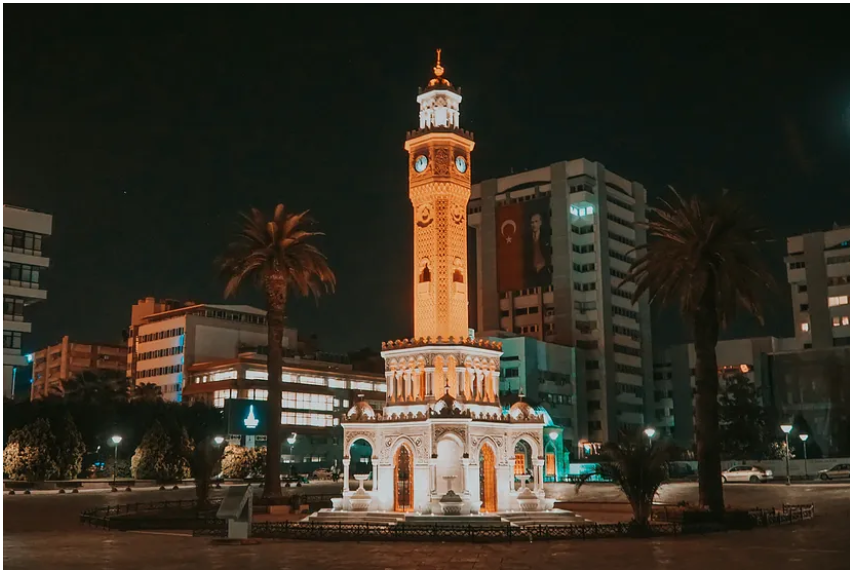
\includegraphics{convex3.png}
			\end{figure}
			\pagebreak
			Resmimize 2 x 2'lik bir ortaklama işlemi yapıyoruz. Bu noktada resmimizi ikiye ikilik parsellere bölüyoruz. Bu işlemden sonra her parseldeki en büyük piksel değerini alıyoruz. Bu işlemi her ayırdığımız parsele uygularsak ortaklama işlemini gerçekleştirmiş oluyoruz. Bu sayede resmimizin boyutu azalmış oluyor ve işlem yükümüzü neredeyse 2 kat düşürmüş oluyoruz. Aynı zamanda çok daha fazla resmi bilgisayarımıza öğretme imkanı bulabiliyoruz.
			\begin{figure}
				\centering
				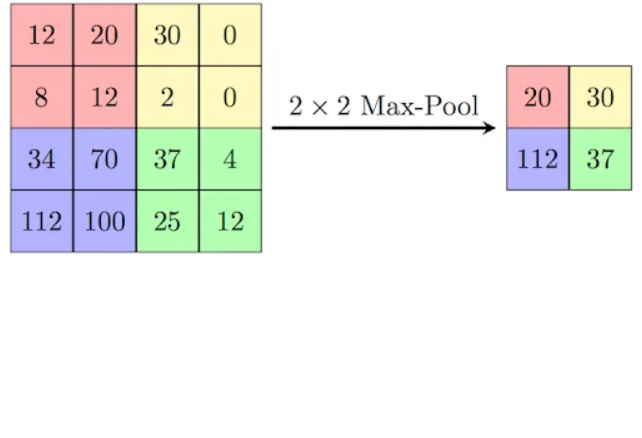
\includegraphics{maxpool.png}
			\end{figure}
			
		\end{enumerate}
		
		\end{center}
		\begin{enumerate}
			\begin{figure}
				\centering
				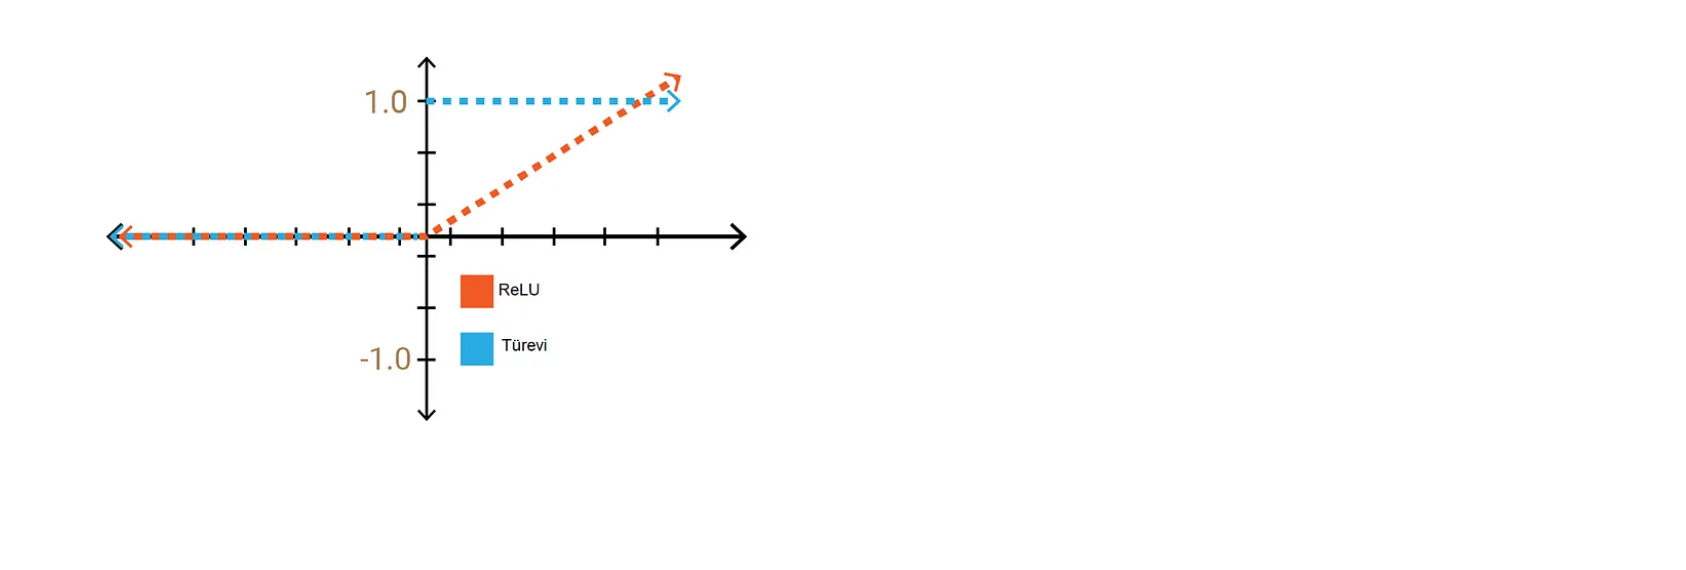
\includegraphics{relu.png}
			\end{figure}
			\item ReLU (Rectified Linear Unit), yapay sinir ağlarında yaygın olarak kullanılan bir aktivasyon fonksiyonudur. Matematiksel olarak, ReLU fonksiyonu aşağıdaki şekilde tanımlanır:
			\[ f(x) = \max(0, x) \]
			
			Bu fonksiyon, giriş değeri 
			x negatif ise sıfır, pozitif ise 			
			x değerini çıktı olarak verir. Yani ReLU fonksiyonu, giriş değerlerini sıfır veya pozitif değerlerle sınırlar.			
			ReLU'nun getirileri ve götürüleri şu şekilde özetlenebilir:
			\vspace{\baselineskip}
			\clearpage
			Getirileri:
			
			Basitlik: ReLU, hesaplama açısından basit bir yapısı olan doğrusal bir fonksiyondur.
			Hız: ReLU, negatif girişlerde sıfır olduğu için diğer aktivasyon fonksiyonlarına kıyasla daha hızlı bir şekilde hesaplanabilir.
			Seyrek Aktivasyon: ReLU'nun negatif bölgesinde sıfır olduğu için, ağın belirli nöronları sık sık aktive olurken diğerleri pasif kalabilir. Bu, ağın daha az kaynak tüketmesini sağlar.
			\vspace{\baselineskip}
			Götürüleri:	
			Sıfır Türev: ReLU'nun negatif bölgesindeki türevi sıfırdır. Bu durum, geriye yayılım algoritmasının eğitimini zorlaştırabilir, çünkü ağın bu bölgesinde öğrenme gerçekleşmez.
			Sıfır Merkezli Problemi: ReLU'nun negatif bölgesinde sıfır olduğu için, bazı nöronlar eğitim sırasında hiç aktive olmayabilir. Bu da ağın öğrenme yeteneğini olumsuz etkileyebilir.
			Genel olarak, ReLU yaygın olarak kullanılan bir aktivasyon fonksiyonudur ve birçok durumda iyi sonuçlar verir. Ancak, özellikle sıfır merkezli probleminin olduğu durumlarda dikkatli kullanılmalıdır.
			\pagebreak
			\item Softmax :
			softmax fonksiyonu, genellikle çoklu sınıf sınıflandırma problemlerinde çıkış katmanında kullanılan bir aktivasyon fonksiyonudur. Sigmoid fonksiyonuna benzer şekilde, girdiyi 0 ile 1 arasında olasılık değerlerine dönüştürür. Ancak softmax fonksiyonu, sınıf sayısına göre bir çıktı vektörü oluşturur ve bu vektördeki her bir değer, girdinin belirli bir sınıfa ait olma olasılığını temsil eder.
			\vspace{\baselineskip}
			$\text{softmax}(z)_i = \frac{e^{z_i}}{\sum_{j=1}^{K} e^{z_j}}$
			\begin{enumerate}
				\item Olasılıksal Yorumlama: Softmax fonksiyonu, giriş vektörünü olasılık dağılımına dönüştürür. Her bir sınıfın olasılığı, giriş vektöründeki ilgili elemanın softmax çıktısına karşılık gelir.
				\item Sınıf Seçimi: Softmax çıktı vektöründe en yüksek olasılığa sahip sınıf genellikle tahmin edilen sınıf olarak seçilir. Bu nedenle, softmax çıktısı, modele göre en olası sınıfı belirlemek için kullanılabilir.
				\item Genelleme: Softmax fonksiyonu, ikiden fazla sınıfı olan sınıflandırma problemlerinde genellikle tercih edilir. Bu fonksiyon, sınıf sayısına göre esnek bir şekilde genelleştirilebilir.
			\end{enumerate}
			
			\begin{minipage}{0.45\textwidth}
				\centering
				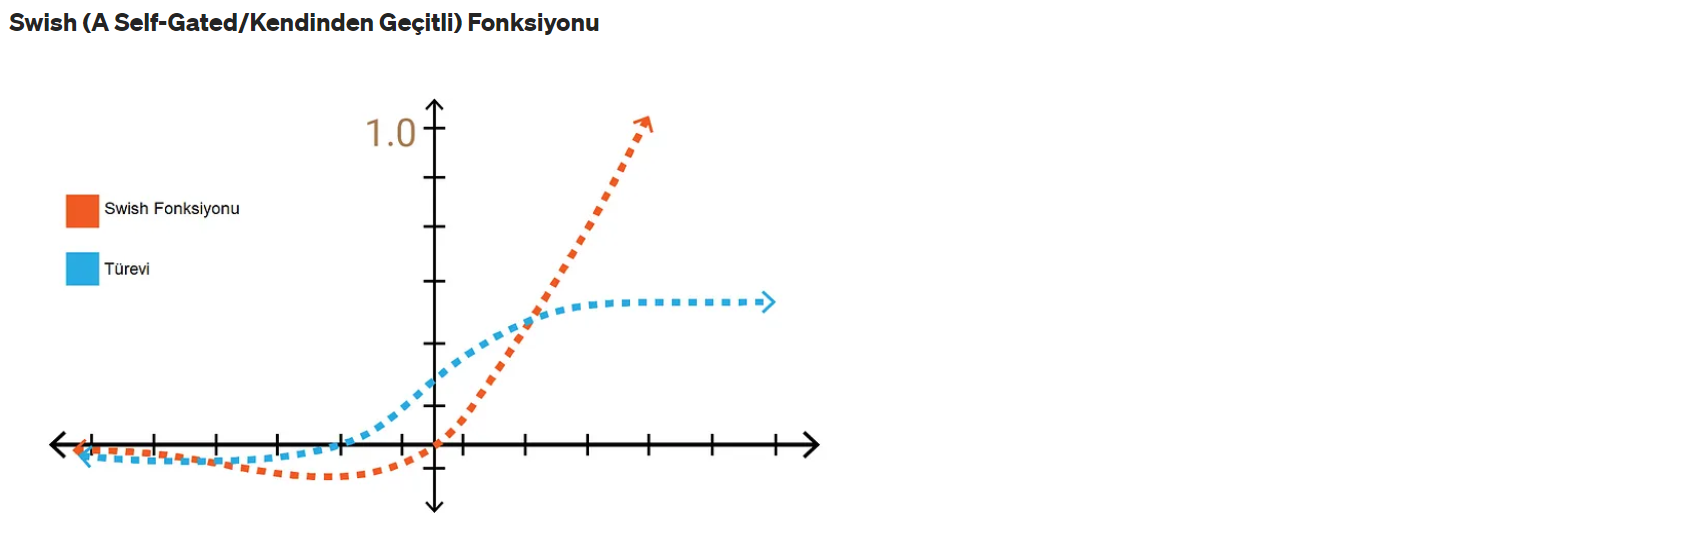
\includegraphics[height=0.5\textheight]{softmax.png}
			\end{minipage}
			
		\end{enumerate}
		\pagebreak
\begin{center}
	\section*{Ubuntu Tensorflow Lite Kurulum }
\end{center}	 

	\begin{enumerate}
		\item Bazelisk Kurulumu
		\begin{verbatim}
			cmake -D CMAKE_BUILD_TYPE=RELEASE -D
		\end{verbatim} 
			\begin{verbatim}
			CMAKE_INSTALL_PREFIX=/usr/local -D WITH_TBB=ON -D
		\end{verbatim}
		\begin{verbatim}
			 BUILD_NEW_PYTHON_SUPPORT=ON -D WITH_V4L=ON -D
			 INSTALL_C_EXAMPLES=ON -D INSTALL_PYTHON_EXAMPLES=ON -D 
		\end{verbatim}
		\begin{verbatim}
			BUILD_EXAMPLES=ON -D WITH_QT=ON -D WITH_GTK=ON -D WITH_OPENGL=ON ..
		\end{verbatim}
		 \item python ./configure.py
		 bazel build -c opt //tensorflow/lite:libtensorflowlite.so
		
		
		
		\item CmakeList hatalı olduğu için kodunu değiştiriyoruz.
		
		
		
		\item 		Git kullanarak TensorFlow deposunu klonlayın ve TensorFlow deposunun içine gidin.
		
		\begin{verbatim}
			git clone https://github.com/tensorflow/tensorflow.git
			cd tensorflow
		\end{verbatim}
		\item Çevresel Değişkenlerin Kurulumu (İsteğe Bağlı):
		Paket oluşturmadan önce çevresel değişkenleri ayarlamak için terminalde aşağıdaki komutları çalıştırın:
		\begin{verbatim}
		
		\end{verbatim}
		\item TensorFlow'u Derlemek:
		Bazel'i kullanarak TensorFlow'u derleyin.
		\begin{verbatim}
			bazel build //tensorflow/tools/pip_package:build_pip_package
		\end{verbatim}
		\item Pip Paketini Oluşturmak ve Yüklemek:
		Oluşturulan .whl dosyasını kullanarak TensorFlow pip paketini oluşturun ve yükleyin.
		\begin{verbatim}
			bazel-bin\tensorflow\tools\pip_package\build_pip_package
		   
		    C:/tmp/tensorflow_pkg
			pip3 install C:/tmp/tensorflow_pkg/tensorflow-<version>.whl
		\end{verbatim}
		
		\item CmakeListi düzenliyoruz
		\begin{verbatim}
			cmake_minimum_required(VERSION 3.2)
			project(tf_test)
			
			set(CMAKE_CXX_STANDARD 14)
			
			# Set paths to directories
			set(distribution_DIR ${CMAKE_SOURCE_DIR}/distribution)
			set(source_DIR ${CMAKE_SOURCE_DIR}/src)
			
			find_package( OpenCV REQUIRED )
			include_directories( ${OpenCV_INCLUDE_DIRS} )
			
			# Define imported libraries
			add_library(libtensorflowlite SHARED IMPORTED)
			add_library(libopencv_core SHARED IMPORTED)
			add_library(libopencv_highgui SHARED IMPORTED)
			add_library(libopencv_imgcodecs SHARED IMPORTED)
			add_library(libopencv_imgproc SHARED IMPORTED)
			
			# Add executable and specify source files
			add_executable(tf_test ${source_DIR}/main.cpp)
			
			# Set include directories for the entire project
			include_directories(${distribution_DIR}/include)
			
			# Link imported libraries to the executable
			target_link_libraries(tf_test
			libtensorflowlite
			libopencv_core
			libopencv_highgui
			libopencv_imgproc
			libopencv_imgcodecs
			)
			
		\end{verbatim}
		\item Flatbuffer kuruyoruz.
		\begin{verbatim}
			cmake ../../tensorflow/lite/tools/cmake/native_tools/flatbuffers/
		\end{verbatim}
		\item Kütüphaneleri bulamadı bir hata alıyoruz çözüm olarak cmakelisti tekrar düzenliyoruz.
		\begin{verbatim}
			CmakeList dosyasında
			add_library(libopencv_core SHARED IMPORTED)
			add_library(libopencv_highgui SHARED IMPORTED)
			add_library(libopencv_imgcodecs SHARED IMPORTED)
			add_library(libopencv_imgproc SHARED IMPORTED)
			target_link_libraries(tf_test
			libtensorflowlite
			libopencv_core
			libopencv_highgui
			libopencv_imgproc
			libopencv_imgcodecs
			)
				set_target_properties(libopencv_core PROPERTIES IMPORTED_LOCATION
			${distribution_DIR}/lib/libopencv_core.so.4.9.0)
			set_target_properties(libopencv_highgui PROPERTIES IMPORTED_LOCATION
			${distribution_DIR}/lib/libopencv_highgui.so.4.9.0)
			set_target_properties(libopencv_imgcodecs PROPERTIES IMPORTED_LOCATION
			${distribution_DIR}/lib/libopencv_imgcodecs.so.4.9.0)
			set_target_properties(libopencv_imgproc PROPERTIES IMPORTED_LOCATION
			${distribution_DIR}/lib/libopencv_imgproc.so.4.9.0)
			sudo ldconfig -v
		
			
		\end{verbatim}
		
		\pagebreak
		\item kodumuzu çalıştırmak için
		\begin{verbatim}
			./tf_test model2.tflite labels_2.txt example_2.JPG 
		\end{verbatim}
		
	\end{enumerate}

	
	\newpage 
	
	\section*{Referanslar} 
	
	\begin{enumerate}
		\item Bazel Ubuntu kurulumu: \url{https://bazel.build/install/ubuntu?hl=tr}
		\item TensorFlow Lite Linux derleme rehberi: \url{https://www.tensorflow.org/lite/guide/python?hl=tr}
		\item Kod olarak yardım aldığım yer:
		\url{https://chat.openai.com}
		\item github repo
		\url {https://github.com/tensorflow/tensorflow}
	\end{enumerate}
	
		
		
		
	\end{enumerate}
\end{document}
